In the original release of the \mf Drain (DRN) Package a drain is designed to simulate the effects of agricultural drains, springs, and other features that remove water from the aquifer at a rate proportional to the difference between the head in the aquifer and some fixed head or elevation, called the drain elevation, so long as the head in the aquifer is above that elevation. If, however, the aquifer head falls below the drain elevation, then the drain has no effect on the aquifer. The constant of proportionality is called the drain conductance.  This chapter describes a new feature of the \mf DRN Package that allows the drain conductance to gradually increase from zero to the user-specified value as a function of the simulated groundwater head.

\subsection{Theory}

The standard drain equation in \mf is

\begin{align}
	\label{eqn:bcdrnqout}
    	\mli{Qout}_{nb} = \begin{dcases} 
    		0 &h_{n} \le \mli{HDRN}_{nb} \\
    		\mli{CDRN}_{nb} \left( h_{n} - \mli{HDRN}_{nb} \right) &h_{n} > \mli{HDRN}_{nb}
	\end{dcases} ,
\end{align}

\noindent where $\mli{Qout}_{nb}$ is the flow from the aquifer to drain $nb$ (\ulct), $\mli{CDRN}_{nb}$ is the drain conductance (\ulst), $\mli{HDRN}_{nb}$ is the drain elevation (\ul), and $h_{n}$ is the head in the cell containing the drain (\ul). Equation~\ref{eqn:bcdrnqout} rewritten in terms of flow from the drain into aquifer (\ulct), $\mli{QDRN}$, is

\begin{align}
	\label{eqn:bcdrnqdrn}
    	\mli{QDRN}_{nb} = \begin{dcases} 
    		\mli{CDRN}_{nb} \left( \mli{HDRN}_{nb} - h_{n} \right) &h_{n} > \mli{HDRN}_{nb} \\
    		0 &h_{n} \le \mli{HDRN}_{nb}
	\end{dcases} .
\end{align}

The standard DRN Package has been modified to include the option to scale the drain conductance using either linear or cubic scaling. The modified form of the drain equation (eq.~\ref{eqn:bcdrnqdrn}) with linear scaling is

\begin{equation}
	\label{eqn:bcdrnqoutalt0}
	\mli{QDRN}_{nb} = F_{\mli{DRN}_{nb}} \mli{CDRN}_{nb} \left( \mli{ZDRN}_{nb} - h_{n} \right) ,
\end{equation}

\noindent where $\mli{ZDRN}_{nb}$ is the elevation at which drainage discharge begins (\ul), and $F_{\mli{DRN}_{nb}}$ is the linear scaling function (unitless), which accounts for how the conductance of the drain changes with changes in head. Conceptually, the drain conductance changes because the area through which flow occurs depends on the head. The area through which flow occurs increases as the head at the drain increases. The linear scaling function is defined as

\begin{equation}
	\begin{aligned}
		\label{eqn:bcdrnFC}
		F_{\mli{DRN}_{nb}} = \begin{dcases} 
			0 &\phantom{0 <} \Delta h_{n,nb}^{r} \le 0 \\
			\Delta h_{n,nb}^{r}  &0 < \Delta h_{n,nb}^{r} < 1 \\
			1 &\phantom{0 <} \Delta h_{n,nb}^{r} \ge 1
		\end{dcases} ,
	\end{aligned}
\end{equation}

\noindent where $\mli{DDRN}_{nb}$ is the drainage depth (\ul) and the relative drain head difference (\ul) is defined as

\begin{equation}
	\label{eqn:reldrainheaddiff}
	\Delta h_{n,nb}^{r} \equiv \frac{h_n - \mli{ZDRN}_{nb}}{\left| \mli{DDRN}_{nb} \right|} .
\end{equation}

\noindent The elevation at which drainage begins, $\mli{ZDRN}_{nb}$ depends on whether the drainage depth, $\mli{DDRN}_{nb}$, is positive or negative and is calculated as

\begin{align}
	\label{eqn:bcdrnZDRN}
	\mli{ZDRN}_{nb} = \begin{dcases}
		\mli{HDRN}_{nb} - \left| \mli{DDRN}_{nb} \right| &\mli{DDRN}_{nb} < 0, \\
		\mli{HDRN}_{nb} &\mli{DDRN}_{nb} \ge 0
    	\end{dcases} .
\end{align}

\noindent If $\mli{DDRN}_{nb}$ is positive, $\mli{ZDRN}_{nb}$ is the drain elevation just as it is in the standard formulation. If $\mli{DDRN}_{nb}$ is negative, $\mli{ZDRN}_{nb}$ is the drain elevation plus the (negative) drainage depth. If $\mli{DDRN}_{nb}$ is zero, the standard formulation is used. The linear scaling function ($F_{\mli{DRN}_{nb}}$) is shown in figure~\ref{fig:drndischscalef}.

\begin{figure}[!ht]
	\begin{center}
	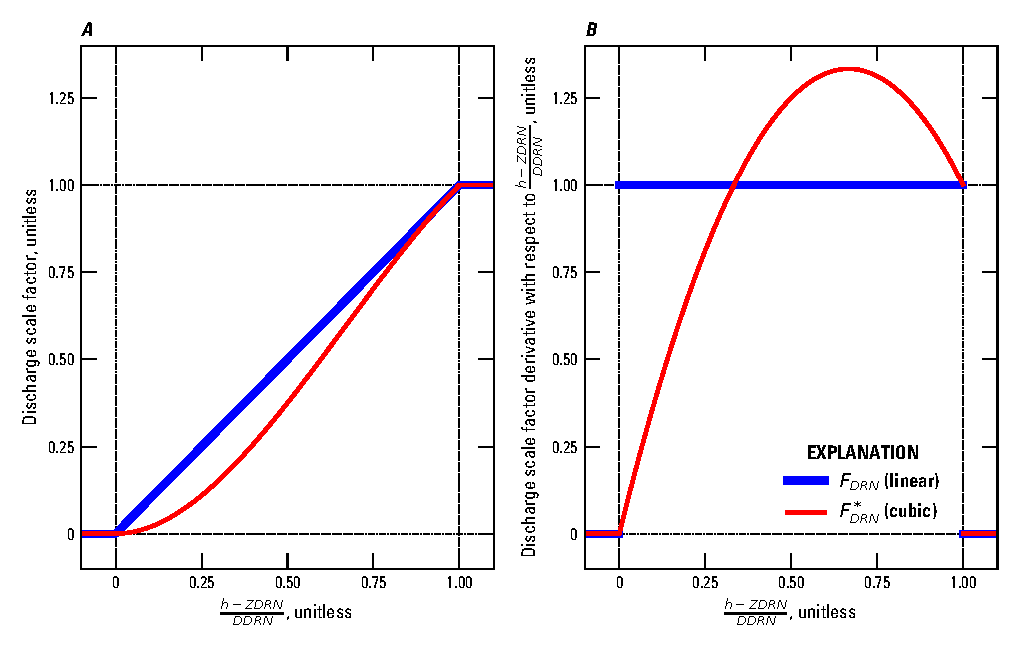
\includegraphics{./Figures/DischargeScaleFactor.pdf}
	\caption[Graphs showing combined linear and cubic scaling functions for drain discharge and the derivatives of the linear and cubic scaling fraction functions]{Graphs showing combined linear and cubic scaling functions for drain discharge and the derivatives of the linear and cubic scaling fraction functions. \textit{A}, linear and cubic fraction functions and \textit{B}, derivatives of the linear and cubic scaling functions with respect to the relative drain head difference $\left( \frac{h - \mli{ZDRN}}{\left| \mli{DDRN} \right|} \right)$. The derivative of the linear and cubic scaling functions with respect to $h$ is the product of the derivative with respect to $\frac{h - \mli{ZDRN}}{\left| \mli{DDRN} \right|}$ and $\frac{1}{\mli{DDRN}}$}
	\label{fig:drndischscalef}
	\end{center}
\end{figure}

The linear scaling function varies with head according to equations~\ref{eqn:bcdrnFC} and~\ref{eqn:reldrainheaddiff}. Differentiation of equation~\ref{eqn:bcdrnFC} with respect to $h_n$, with application of the chain rule to account for the variation of $ \Delta h_{n,nb}^{r}$ with respect to $h_n$ in equation~\ref{eqn:reldrainheaddiff}, gives

\begin{equation}
	\label{eqn:bcdrndFC}
	\begin{aligned}
		\frac{\partial F_{\mli{DRN}_{nb}}}{\partial h_n} = \begin{dcases} 
			0 &\phantom{0 <} \Delta h_{n,nb}^{r} \le 0 \\
			\frac{1}{\left| \mli{DDRN}_{nb} \right|}  &0 < \Delta h_{n,nb}^{r} < 1 \\
			1 &\phantom{0 <} \Delta h_{n,nb}^{r} \ge 1
		\end{dcases} ,
	\end{aligned}
\end{equation}

\noindent which is discontinuous in the neighborhood of $h_n = \mli{ZDRN}_{nb}$ and $h_n = \mli{ZDRN}_{nb} - \left| \mli{DDRN}_{nb} \right| $. The derivative of the linear scaled drain discharge (eq.~\ref{eqn:bcdrnqoutalt0}) with respect to $h_n$ is

\begin{equation}
	\label{eqn:bcdrnNRlindqoutalt0}
	\frac{\partial \mli{QDRN}_{nb}}{\partial h_n} = -F_{\mli{DRN}_{nb}} \mli{CDRN}_{nb}  + \frac{\partial F_{\mli{DRN}_{nb}}}{\partial h_n} \mli{CDRN}_{nb} \left( \mli{ZDRN}_{nb} - h_{n} \right) .
\end{equation}

\noindent Substitution of equations ~\ref{eqn:bcdrnFC} and~\ref{eqn:bcdrndFC} into equation~\ref{eqn:bcdrnNRlindqoutalt0} results in

\begin{equation}
	\begin{aligned}
		\label{eqn:bcdrnNRlindQdh}
		\frac{\partial \mli{QDRN}_{nb}}{\partial h_n} = \begin{dcases} 
			0 &\phantom{0 <} \Delta h_{n,nb}^{r} \le 0 \\
			- 2\, \mli{CDRN}_{nb} \, \Delta h_{n,nb}^{r}  &0 < \Delta h_{n,nb}^{r} < 1 \\
			-\mli{CDRN}_{nb} &\phantom{0 <} \Delta h_{n,nb}^{r} \ge 1
		\end{dcases} ,
	\end{aligned}
\end{equation}

\noindent which remains discontinuous in the vicinity of $\mli{ZDRN}_{nb}$.

When the Newton-Raphson formulation is used, discontinuous derivatives can cause non-convergence in the neighborhood of the discontinuity \citep{doi:10.1029/2006WR005195}. To ensure continuous drain discharge derivatives when the Newton-Raphson formulation is used, cubic smoothing of the linear relative drain head difference is used and equation~\ref{eqn:bcdrnqoutalt0} is modified to

\begin{equation}
	\label{eqn:bcdrnNRqoutalt0}
	\mli{QDRN}_{nb}^* = F_{\mli{DRN}_{nb}}^* \mli{CDRN}_{nb} \left( \mli{ZDRN}_{nb} - h_{n} \right) ,
\end{equation}

\noindent where where $F_{\mli{DRN}_{nb}}^*$ is the cubic scaling function. The cubic scaling function is defined as

\begin{equation}
	\begin{aligned}
		\label{eqn:bcdrnFCC}
		F_{\mli{DRN}_{nb}}^* = \begin{dcases} 
			0 & \phantom{0 <} \Delta h_{n,nb}^{r} \le 0 \\
			- \left( \Delta h_{n,nb}^{r} \right)^3  + 2 \left( \Delta h_{n,nb}^{r} \right)^2  & 0 < \Delta h_{n,nb}^{r} < 1 \\
			1 & \phantom{0 <} \Delta h_{n,nb}^{r} \ge 1
		\end{dcases} ,
	\end{aligned}
\end{equation}

\noindent which is continuous in the vicinity of $h_n = \mli{ZDRN}_{nb}$ and $h_n = \mli{ZDRN}_{nb} - \left| \mli{DDRN}_{nb} \right| $ (fig.~\ref{fig:drndischscalef}\textit{A}). The derivative of equation~\ref{eqn:bcdrnFCC} with respect to $h_n$ is

\begin{equation}
	\begin{aligned}
		\label{eqn:bcdrndFCC}
		\frac{\partial F_{\mli{DRN}_{nb}}^*}{\partial h_n} = \begin{dcases} 
			0 & \phantom{0 <} \Delta h_{n,nb}^{r} \le 0 \\
			-\frac{3}{\left| \mli{DDRN}_{nb} \right|} \left( \Delta h_{n,nb}^{r} \right)^2  + \\
			\phantom{-}\frac{4}{\left| \mli{DDRN}_{nb} \right|} \, \Delta h_{n,nb}^{r} & 0 < \Delta h_{n,nb}^{r} < 1 \\
			0 & \phantom{0 <} \Delta h_{n,nb}^{r} \ge 1
		\end{dcases} ,
	\end{aligned}
\end{equation}

\noindent which is discontinuous in the vicinity of $h_n = \mli{ZDRN}_{nb} - \left| \mli{DDRN}_{nb} \right| $ (fig.~\ref{fig:drndischscalef}\textit{B}). The derivative of the cubic scaled drain discharge (eq.~\ref{eqn:bcdrnNRqoutalt0}) with respect to $h$ is

\begin{equation}
	\label{eqn:bcdrnNRdqoutalt0}
	\frac{\partial \mli{QDRN}_{nb}^*}{\partial h} = -F_{\mli{DRN}_{nb}}^* \mli{CDRN}_{nb}  + \frac{\partial F_{\mli{DRN}_{nb}}^*}{\partial h} \mli{CDRN}_{nb} \left( \mli{ZDRN}_{nb} - h_{n} \right) .
\end{equation}

\noindent Substitution of equations~\ref{eqn:bcdrnFCC} and~\ref{eqn:bcdrndFCC} into equation~\ref{eqn:bcdrnNRdqoutalt0} results in 

\begin{equation}
	\begin{aligned}
		\label{eqn:bcdrndQdh}
		\frac{\partial \mli{QDRN}_{nb}^*}{\partial h_n} = \begin{dcases} 
			0 & \phantom{0 <} \Delta h_{n,nb}^{r} \le 0 \\
			-\mli{CDRN}_{nb} \Biggl[ - \left( \Delta h_{n,nb}^{r} \right)^3  + 2 \left( \Delta h_{n,nb}^{r} \right)^2 \Biggr] + \\
			\phantom{-} \mli{CDRN}_{nb} \Biggl[- \frac{3}{\mli{DDRN}_{nb}} \left( \Delta h_{n,nb}^{r} \right)^2  + \Biggr. \\
			\Biggl. \phantom{-\mli{CDRN}_{nb} \Biggl[- } \frac{4}{\mli{DDRN}_{nb}} \left( \Delta h_{n,nb}^{r} \right) \Biggr] \left( \mli{ZDRN}_{nb} - h_{n} \right) & 0 < \Delta h_{n,nb}^{r} < 1 \\
			-\mli{CDRN}_{nb} & \phantom{0 <} \Delta h_{n,nb}^{r} \ge 1
		\end{dcases} ,
	\end{aligned}
\end{equation}

\noindent which is continuous in the vicinity of $h_n = \mli{ZDRN}_{nb}$ and $h_n = \mli{ZDRN}_{nb} - \left| \mli{DDRN}_{nb} \right| $.

\subsection{Example Drain Discharge Scaling Calculations}

An example of the differences between the standard, linearly-scaled, and cubicly-scaled drainage discharge are shown in figure~\ref{fig:drndischdiff}. In this example the elevation that drainage discharge starts ($\mli{ZDRN}$) is set at $\frac{\mli{DDRN}}{2}$ below land surface elevation and drainage discharge is equal for all approaches at $\mli{ZDRN} + \mli{DDRN}$ (fig.~\ref{fig:drndischdiff}\textit{A}). In this conceptual problem, the groundwater head linearly increases from a value less than $\mli{ZDRN}$ to greater than $\mli{ZDRN + DDN}$ during the simulation, which is presented as the head difference ($h - \mli{ZDRN}$) divided by the drainage depth in figure~\ref{fig:drndischdiff}\textit{B}. The drainage discharge that results from the linear increase in groundwater head using the original-, linear-, and cubic-scaling increases with time as is shown in figure~\ref{fig:drndischdiff}\textit{C} and shows the continuous nature of the linear- and cubic scaled drainage discharge and that all three approaches result in the same drain discharge rate when the relative drain head difference is greater than or equal to one. Figure~\ref{fig:drndischdiff}\textit{D} shows that the cumulative drain discharge for the original drain formulation is 170 to 200 $L^3$ greater than the cubic- and linear-scaled drainage discharge, respectively.

\begin{figure}[!ht]
	\begin{center}
	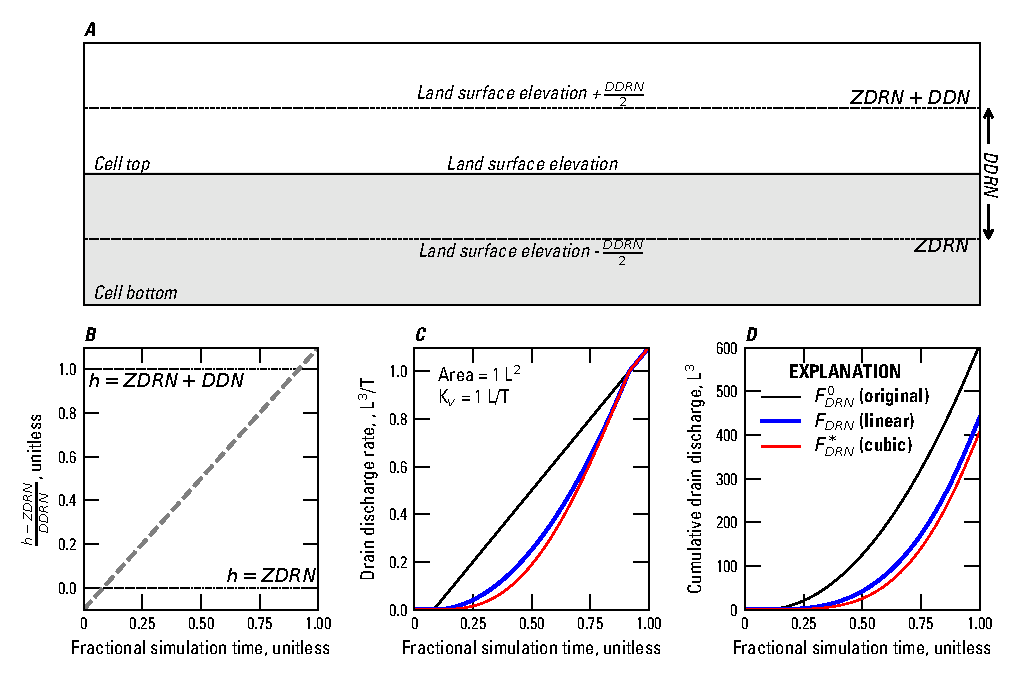
\includegraphics{./Figures/DRNDischargeDifferences.pdf}
	\caption[Graphs showing a conceptual model cell using scaled drain discharge and the relation between the groundwater level and drain discharge]{Graphs showing a conceptual model cell using scaled drain discharge and the relation between the groundwater level and drain discharge. \textit{A}, Conceptual model cell containing a drain cell where drainage discharge starts $\frac{\mli{DDRN}}{2}$ below land surface and is equal $\frac{\mli{DDRN}}{2}$ above land surface for all drain scaling approaches, \textit{B}, conceptual linear groundwater level increases, which are presented as a relative drain head difference, with fractional simulation time, \textit{C}, calculated original, linear, and cubic scaled drainage discharge rates resulting from conceptual groundwater level increases, and \textit{D}, calculated original, linear, and cubic scaled drainage cumulative discharge resulting from conceptual groundwater level increases}
	\label{fig:drndischdiff}
	\end{center}
\end{figure}

\subsection{Incorporation of the modified Drain (DRN) Package into the CVFD Groundwater Flow Equation}

To prepare the CVFD equation for solution using the standard formulation, it is convenient to rearrange the discretized groundwater flow equation for a cell so that all terms containing heads at the end of the current time step are grouped on the left-hand side of the equation, and all terms that are independent of head at the end of the current time step are on the right-hand side of equation 6--1 in \cite{modflow6gwf}. Refer to \cite{modflow6gwf} for additional information on how the groundwater flow equation is formulated in \mf. 

\subsubsection{Standard Formulation}

According to the sign convention in \mf, $\mli{QDRN}_{nb}$ in the groundwater flow equation is defined as a head-dependent flow out of cell $n$, and corresponding terms must be added to the left and right sides of equation~6--1 in \cite{modflow6gwf} for each cell containing a drain. This is accomplished in the modified Drain Package by adding the head-dependent term and the known term in equation~\ref{eqn:bcdrnqoutalt0} to the left- and right-side of equation~6--1 in \cite{modflow6gwf}. The contribution of the modified drain equations to the left-hand side and right-hand sides of the groundwater flow equation are

\begin{equation}
	\label{eqn:qdrnstd}
	\begin{aligned}
		A_{n,n} &\leftarrow A_{n,n} - F_{\mli{DRN}_{nb}} \mli{CDRN}_{nb}   \\
		b_n &\leftarrow b_n - F_{\mli{DRN}_{nb}} \mli{CDRN}_{nb} ZDRN_{nb} ,
	\end{aligned}
\end{equation} 

\noindent where $A_{n,n}$ is the diagonal of the coefficient matrix for cell $n$ and $b_n$ is the right-hand side of the groundwater flow equation for cell $n$. In the case where drainage discharge is not scaled, $F_{\mli{DRN}_{nb}}$ is zero when $h_n$ is less than or equal to $HDRN_{nb}$ and one when $h_n$ is greater than $HDRN_{nb}$, which results in identical behavior as the original drain package formulation.


\subsubsection{Newton-Raphson Formulation}

The modified Newton-Raphson form of equation~\ref{eqn:bcdrnNRqoutalt0} solved in terms of $h$ instead of $\Delta h$  and incorporated into the Newton-Raphson form of the groundwater flow equation \citep[eq. 2--26]{modflow6gwf} is

\begin{equation}
	\label{eqn:nrQout}
	\frac{\partial \mli{QDRN}_{nb}^*}{\partial h_n}  h^k_n  = - \mli{QDRN}_{nb}^* + 
	\frac{\partial \mli{QDRN}_{nb}^*}{\partial h_n}  h^{k-1}_n,
\end{equation} 

\noindent where $h^k_n$ is the head at the end of the current non-linear (picard) iteration and $h^{k-1}_n$ is the head at the start of the current non-linear iteration. Substitution of equations~\ref{eqn:bcdrnNRqoutalt0} and~\ref{eqn:bcdrnNRdqoutalt0} into equation~\ref{eqn:nrQout} results in

\begin{equation}
	\label{eqn:nrQout01}
	\begin{aligned}
		A_{n,n} \leftarrow & A_{n,n} - F_{\mli{DRN}_{nb}}^* \mli{CDRN}_{nb}  + \frac{\partial F_{\mli{DRN}_{nb}}^*}{\partial h} \mli{CDRN}_{nb} \left( \mli{ZDRN}_{nb} - h_{n} \right) \\
		b_n \leftarrow & b_n - F_{\mli{DRN}_{nb}}^* \mli{CDRN}_{nb} \left( \mli{ZDRN}_{nb} - h_{n}^{k-1} \right) \\
		& \phantom{b_n} + \Biggl[ -F_{\mli{DRN}_{nb}}^* \mli{CDRN}_{nb} + \frac{\partial F_{\mli{DRN}_{nb}}^*}{\partial h} \mli{CDRN}_{nb} \left( \mli{ZDRN}_{nb} - h_{n} \right) \Biggr] h^{k-1}_n .
	\end{aligned} 
\end{equation}

\noindent Simplifying the right-hand side contribution in equation~\ref{eqn:nrQout01} results in

\begin{equation}
	\label{eqn:nrQout02}
	b_n \leftarrow b_n - F_{\mli{DRN}_{nb}}^* \mli{CDRN}_{nb} \mli{ZDRN}_{nb} + \Biggl[ \frac{\partial F_{\mli{DRN}_{nb}}^*}{\partial h} \mli{CDRN}_{nb} \left( \mli{ZDRN}_{nb} - h_{n}  \right) \Biggr] h^{k-1}_n .
\end{equation}

\noindent The $F_{\mli{DRN}_{nb}}^* \mli{CDRN}_{nb}$ term in equation~\ref{eqn:nrQout01} and the $F_{\mli{DRN}_{nb}}^* \mli{CDRN}_{nb} \mli{ZDRN}_{nb}$ term in equation~\ref{eqn:nrQout02} are subtracted from the diagonal of the coefficient matrix and the right-hand side of the groundwater-flow equation, respectively, during the standard formulation step for the drain package. The Newton-Raphson formulation for the modified drain package is completed by augmenting the coefficient matrix with the derivative term in equation~\ref{eqn:nrQout01} and adding the second term in equation~\ref{eqn:nrQout02} (the product of a derivative term and the head at the start of the current iteration) to the right-hand side of the groundwater-flow equation. 

\subsection{Use of Drain Discharge Scaling}

A few examples of how the modified drain package can be used to simulate drainage discharge consistent with other \mf packages are given below.

\paragraph{The original drain package formulation with a specified drainage depth value}

Specifying $\mli{DDRN}$ to be 0 results in a drain that behaves the same as the original DRN Package (eq.~\ref{eqn:bcdrnqout}). Using a combination of $\mli{DDRN}$ values set to zero and non-zero values will result in drains with 0 values behaving like the original drain package and others using the scaled drainage discharge approach.

\paragraph{Groundwater seepage from the Unsaturated Zone Flow Package}

The drain package can be used as an alternative to the groundwater seepage option in the Unsaturated Zone Flow (UZF) Package. Specifying a positive $\mli{DDRN}$ value and $\mli{HDRN}_{nb}$ to be $\frac{\mli{DDRN}}{2}$ below the single values specified with the standard DRN Package approach (for example, setting $\mli{DDRN}$ to be at land surface) results in a formulation that is equivalent to the groundwater seepage option available in the UZF Package in \mf \citep{modflow6gwf}. To be consistent with the UZF package, the drain conductance should be calculated as

\begin{equation}
	\label{eqn:uzfcond}
	\mli{CDRN}_{nb} = \frac{K_{v_{nb}} A_n}{\mli{DDRN}_{nb}} ,
\end{equation}

\noindent where $K_{v_{nb}}$ is vertical hydraulic conductivity (\ult) and $A_n$ is the horizontal area of cell $n$ (\uls).
